\section{Kết quả và Kết luận}

\subsection{Kết quả Phân tích Khám phá Dữ liệu}

\subsubsection{Thông tin tổng quan về dữ liệu}
Sau quá trình đọc và làm sạch dữ liệu:
\begin{itemize}
	\item \textbf{Tập huấn luyện}: Còn lại 8896 mẫu (đã loại 103 mẫu trùng lặp)
	\item \textbf{Tập kiểm tra}: Còn lại 999 mẫu (đã loại 1 mẫu trùng lặp)
	\item \textbf{Đặc trưng}: 5 đặc trưng đầu vào và 1 biến mục tiêu (Performance Index)
	\item \textbf{Chất lượng dữ liệu}: Không có giá trị thiếu (missing values)
\end{itemize}

\subsubsection{Phân tích trực quan hóa dữ liệu}
Từ 6 biểu đồ được tạo ra trong quá trình EDA:

\begin{figure}[H]
	\centering
	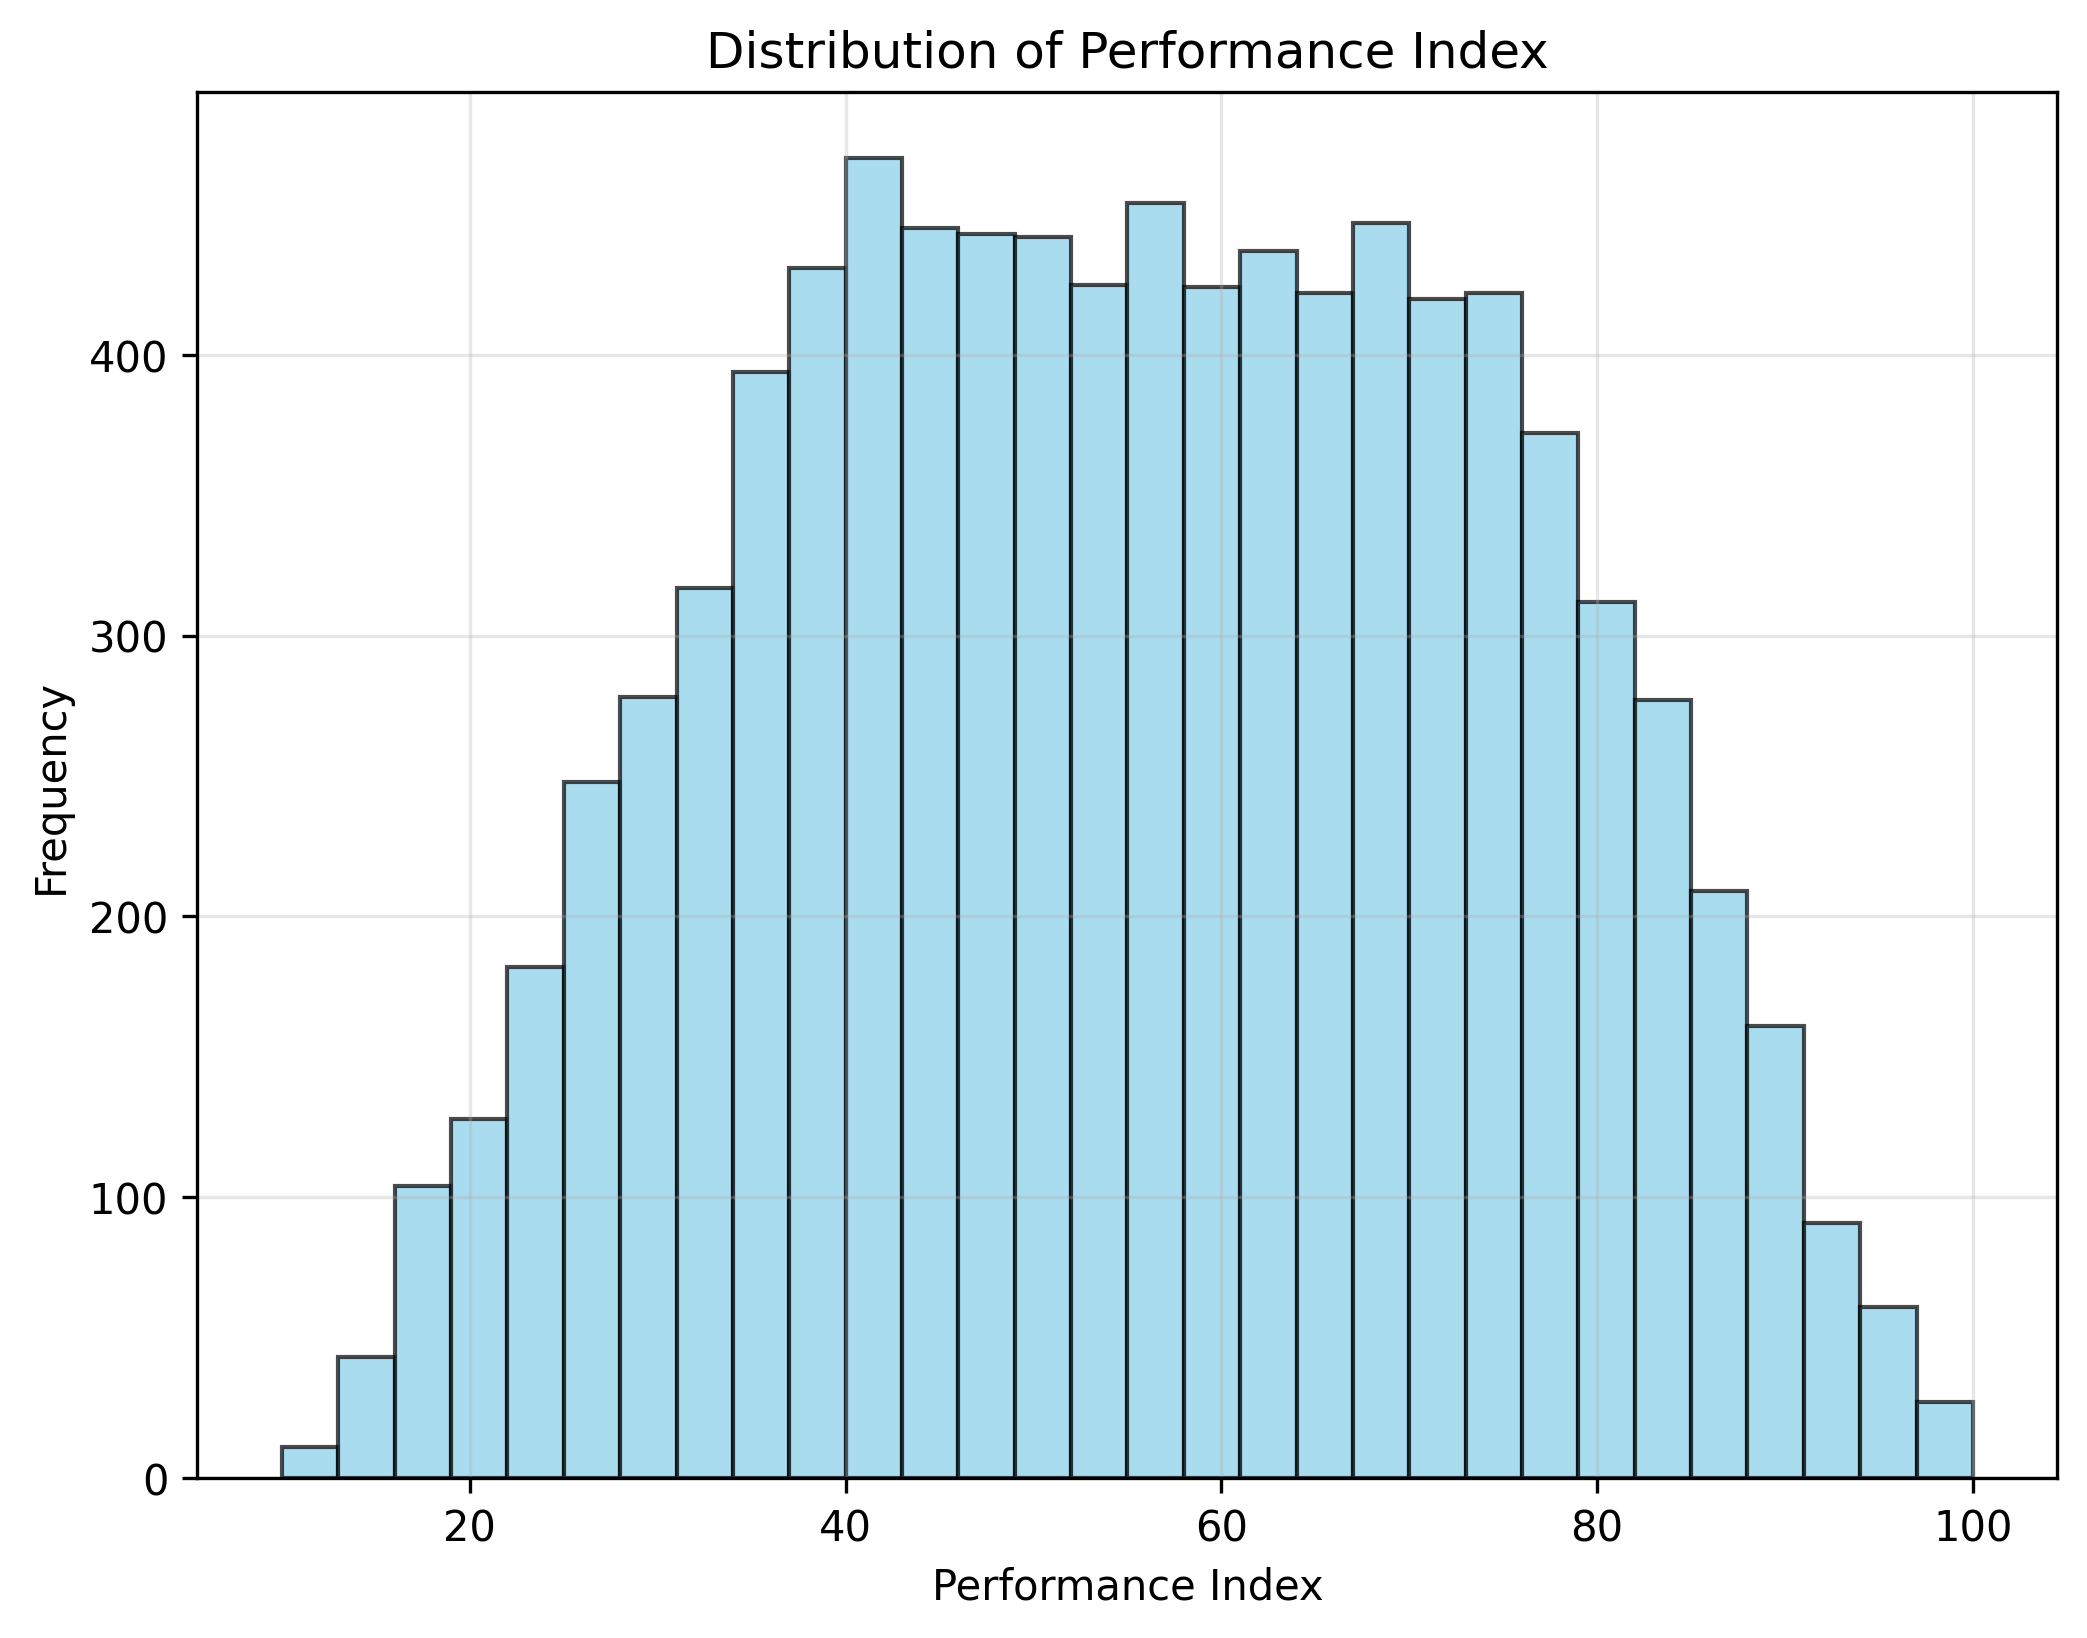
\includegraphics[width=0.7\textwidth]{imgs/figures/figure1_performance_index_distribution.png}
	\caption{Phân phối Performance Index}
	\label{fig:performance_distribution}
\end{figure}

\begin{itemize}
	\item \textbf{Nhận xét:}
	      \begin{itemize}
		      \item \textbf{Phân phối gần chuẩn}: Biểu đồ histogram cho thấy Performance Index có phân phối gần như chuẩn với đỉnh tại khoảng 40-45 điểm.
		      \item \textbf{Tính đối xứng}: Phân phối tương đối đối xứng với độ lệch nhẹ về phía phải.
		      \item \textbf{Phạm vi rộng}: Dữ liệu phân bố từ khoảng 10 đến gần 100 điểm, cho thấy sự đa dạng lớn trong hiệu suất học tập.
		      \item \textbf{Tập trung chính}: Phần lớn sinh viên có điểm số trong khoảng 30-70, với mật độ cao nhất ở khoảng 40-50 điểm.
	      \end{itemize}
\end{itemize}

\begin{figure}[H]
	\centering
	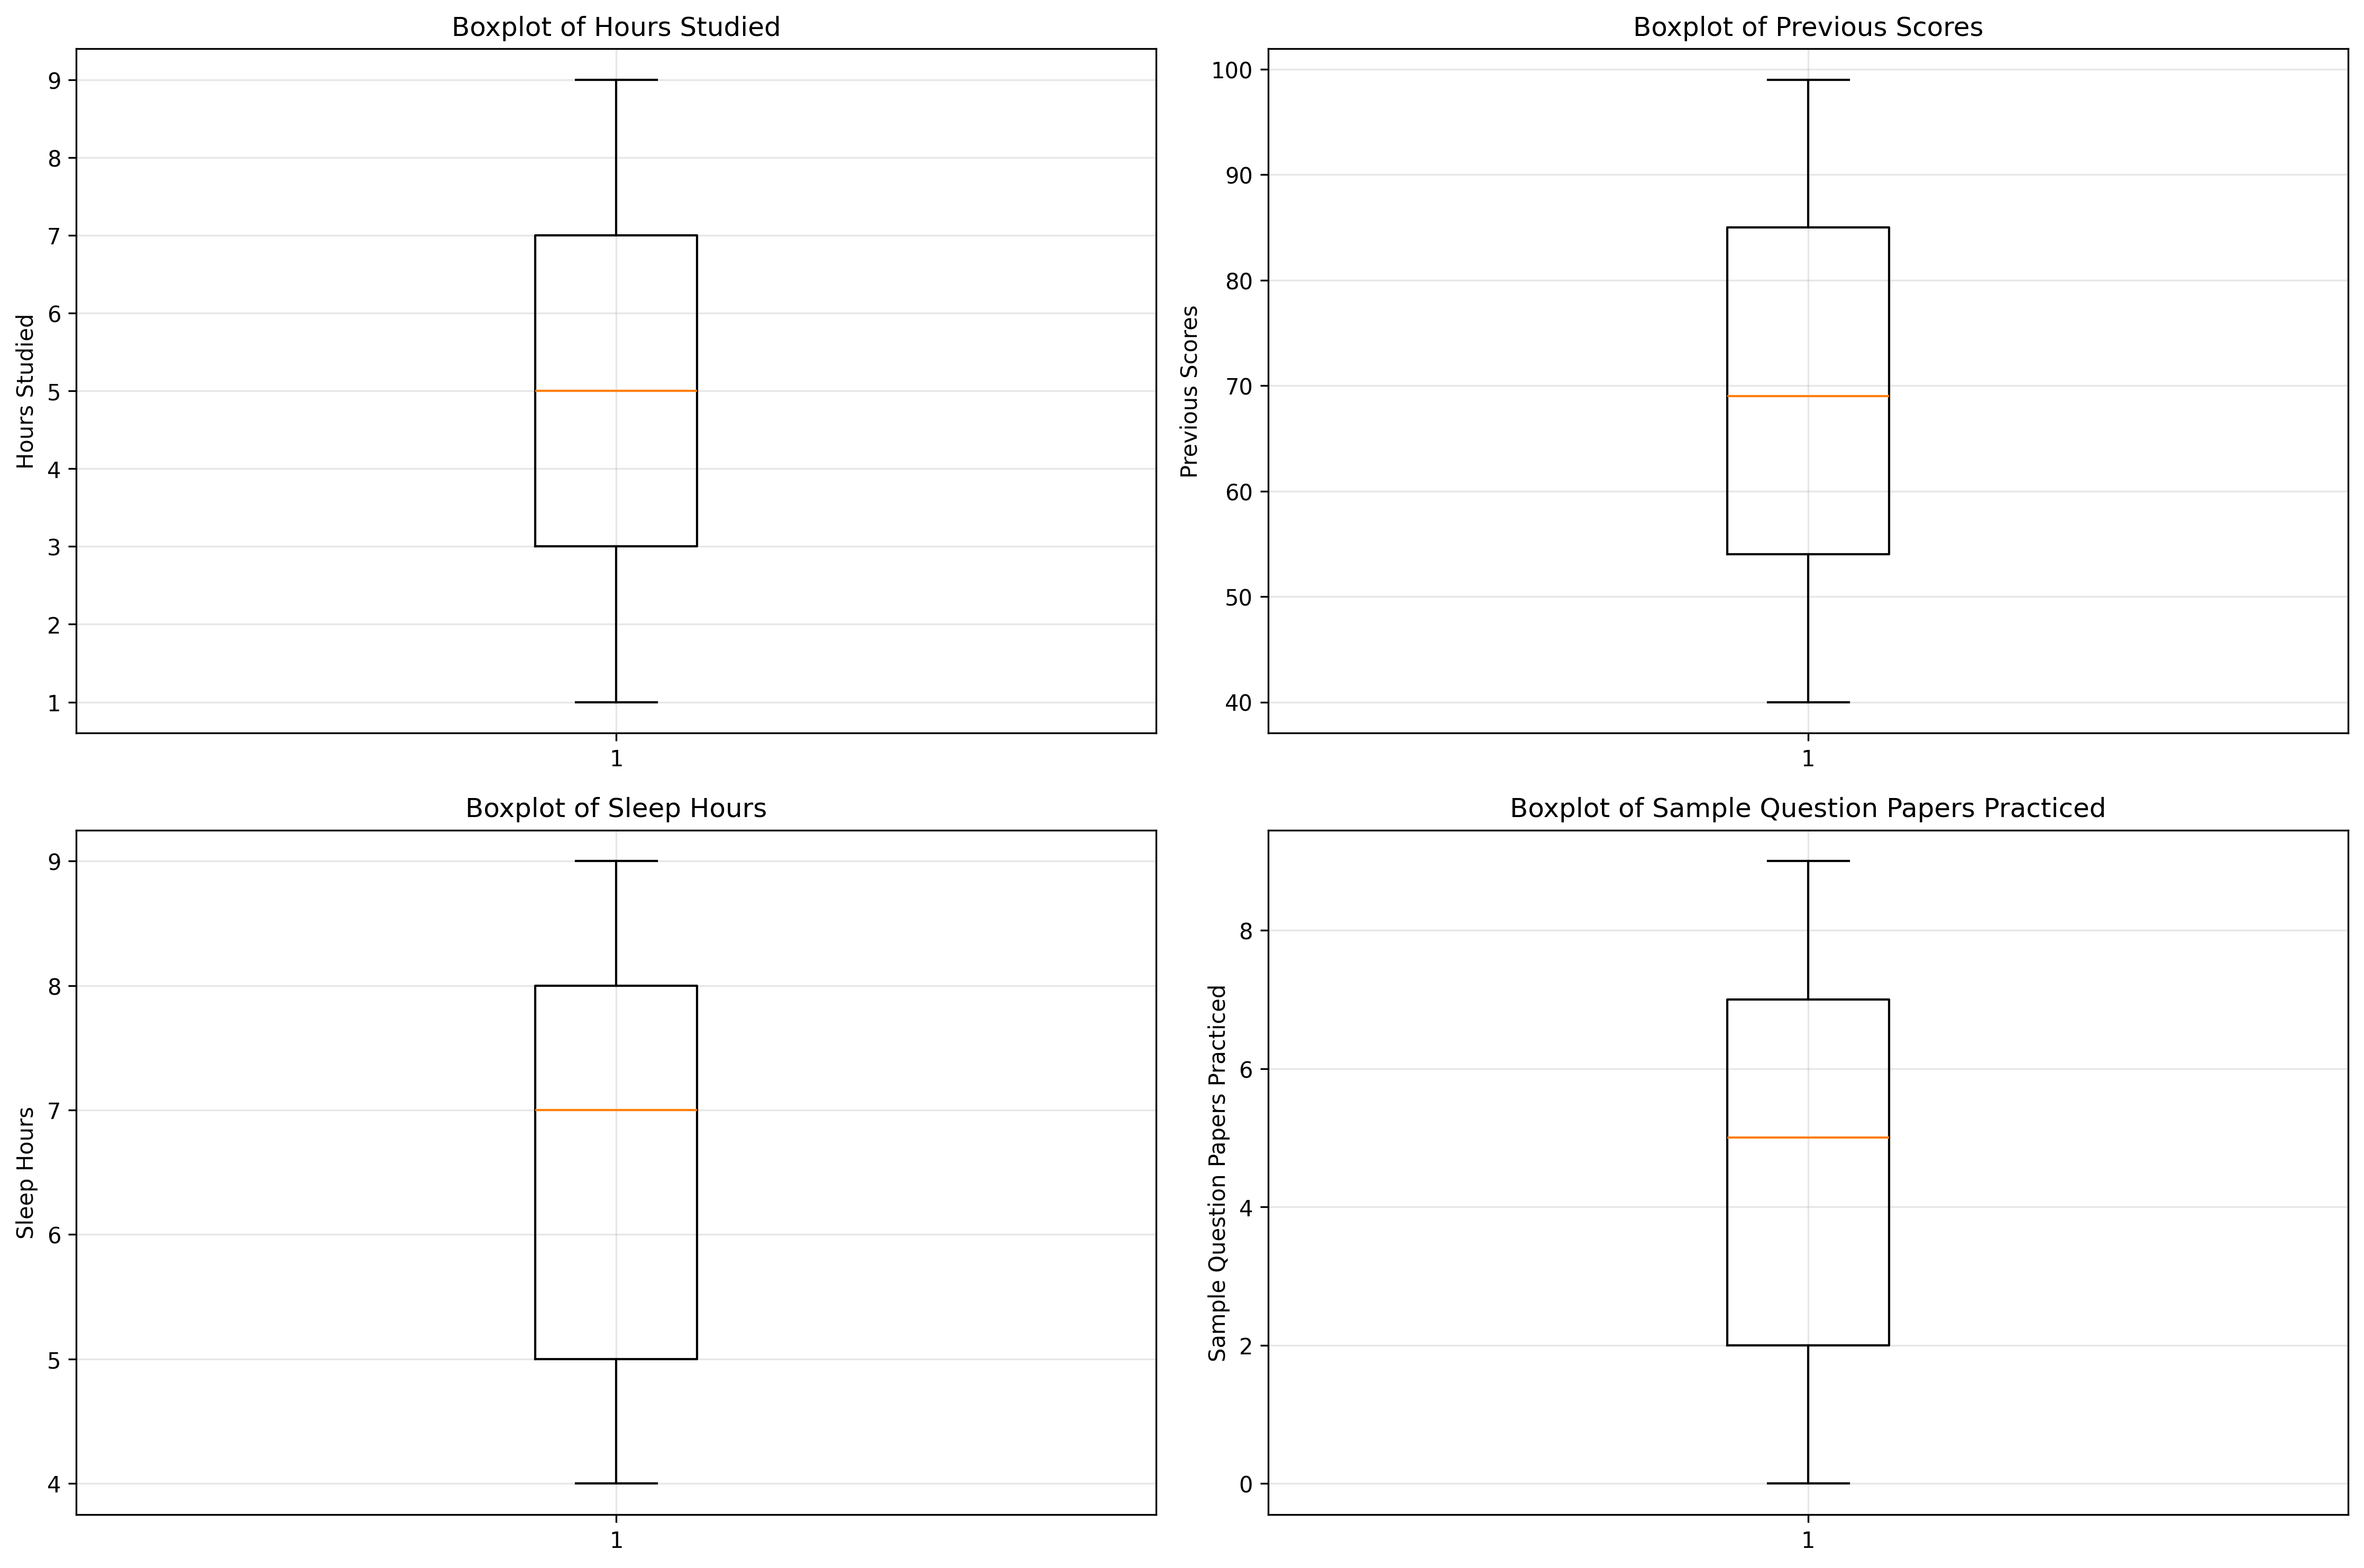
\includegraphics[width=0.9\textwidth]{imgs/figures/figure2_boxplots_numerical_features.png}
	\caption{Biểu đồ hộp các đặc trưng số}
	\label{fig:boxplots}
\end{figure}

\begin{itemize}
	\item \textbf{Nhận xét:}
	      \begin{itemize}
		      \item \textbf{Hours Studied}: Phân phối đối xứng với trung vị khoảng 5 giờ, IQR từ 3-7 giờ, phạm vi từ 1-9 giờ. Không có outliers đáng kể.
		      \item \textbf{Previous Scores}: Phân phối đối xứng với trung vị khoảng 70 điểm, IQR từ 55-85 điểm, phạm vi từ 40-100 điểm. Phân phối cân bằng và ổn định.
		      \item \textbf{Sleep Hours}: Phân phối đối xứng với trung vị khoảng 7 giờ, IQR từ 5-8 giờ, phạm vi từ 4-9 giờ. Phân bố khá tập trung.
		      \item \textbf{Sample Question Papers}: Phân phối đối xứng với trung vị khoảng 5 đề, IQR từ 2-7 đề, phạm vi từ 0-9 đề. Có một số sinh viên không luyện đề (giá trị 0).
	      \end{itemize}
\end{itemize}

\begin{figure}[H]
	\centering
	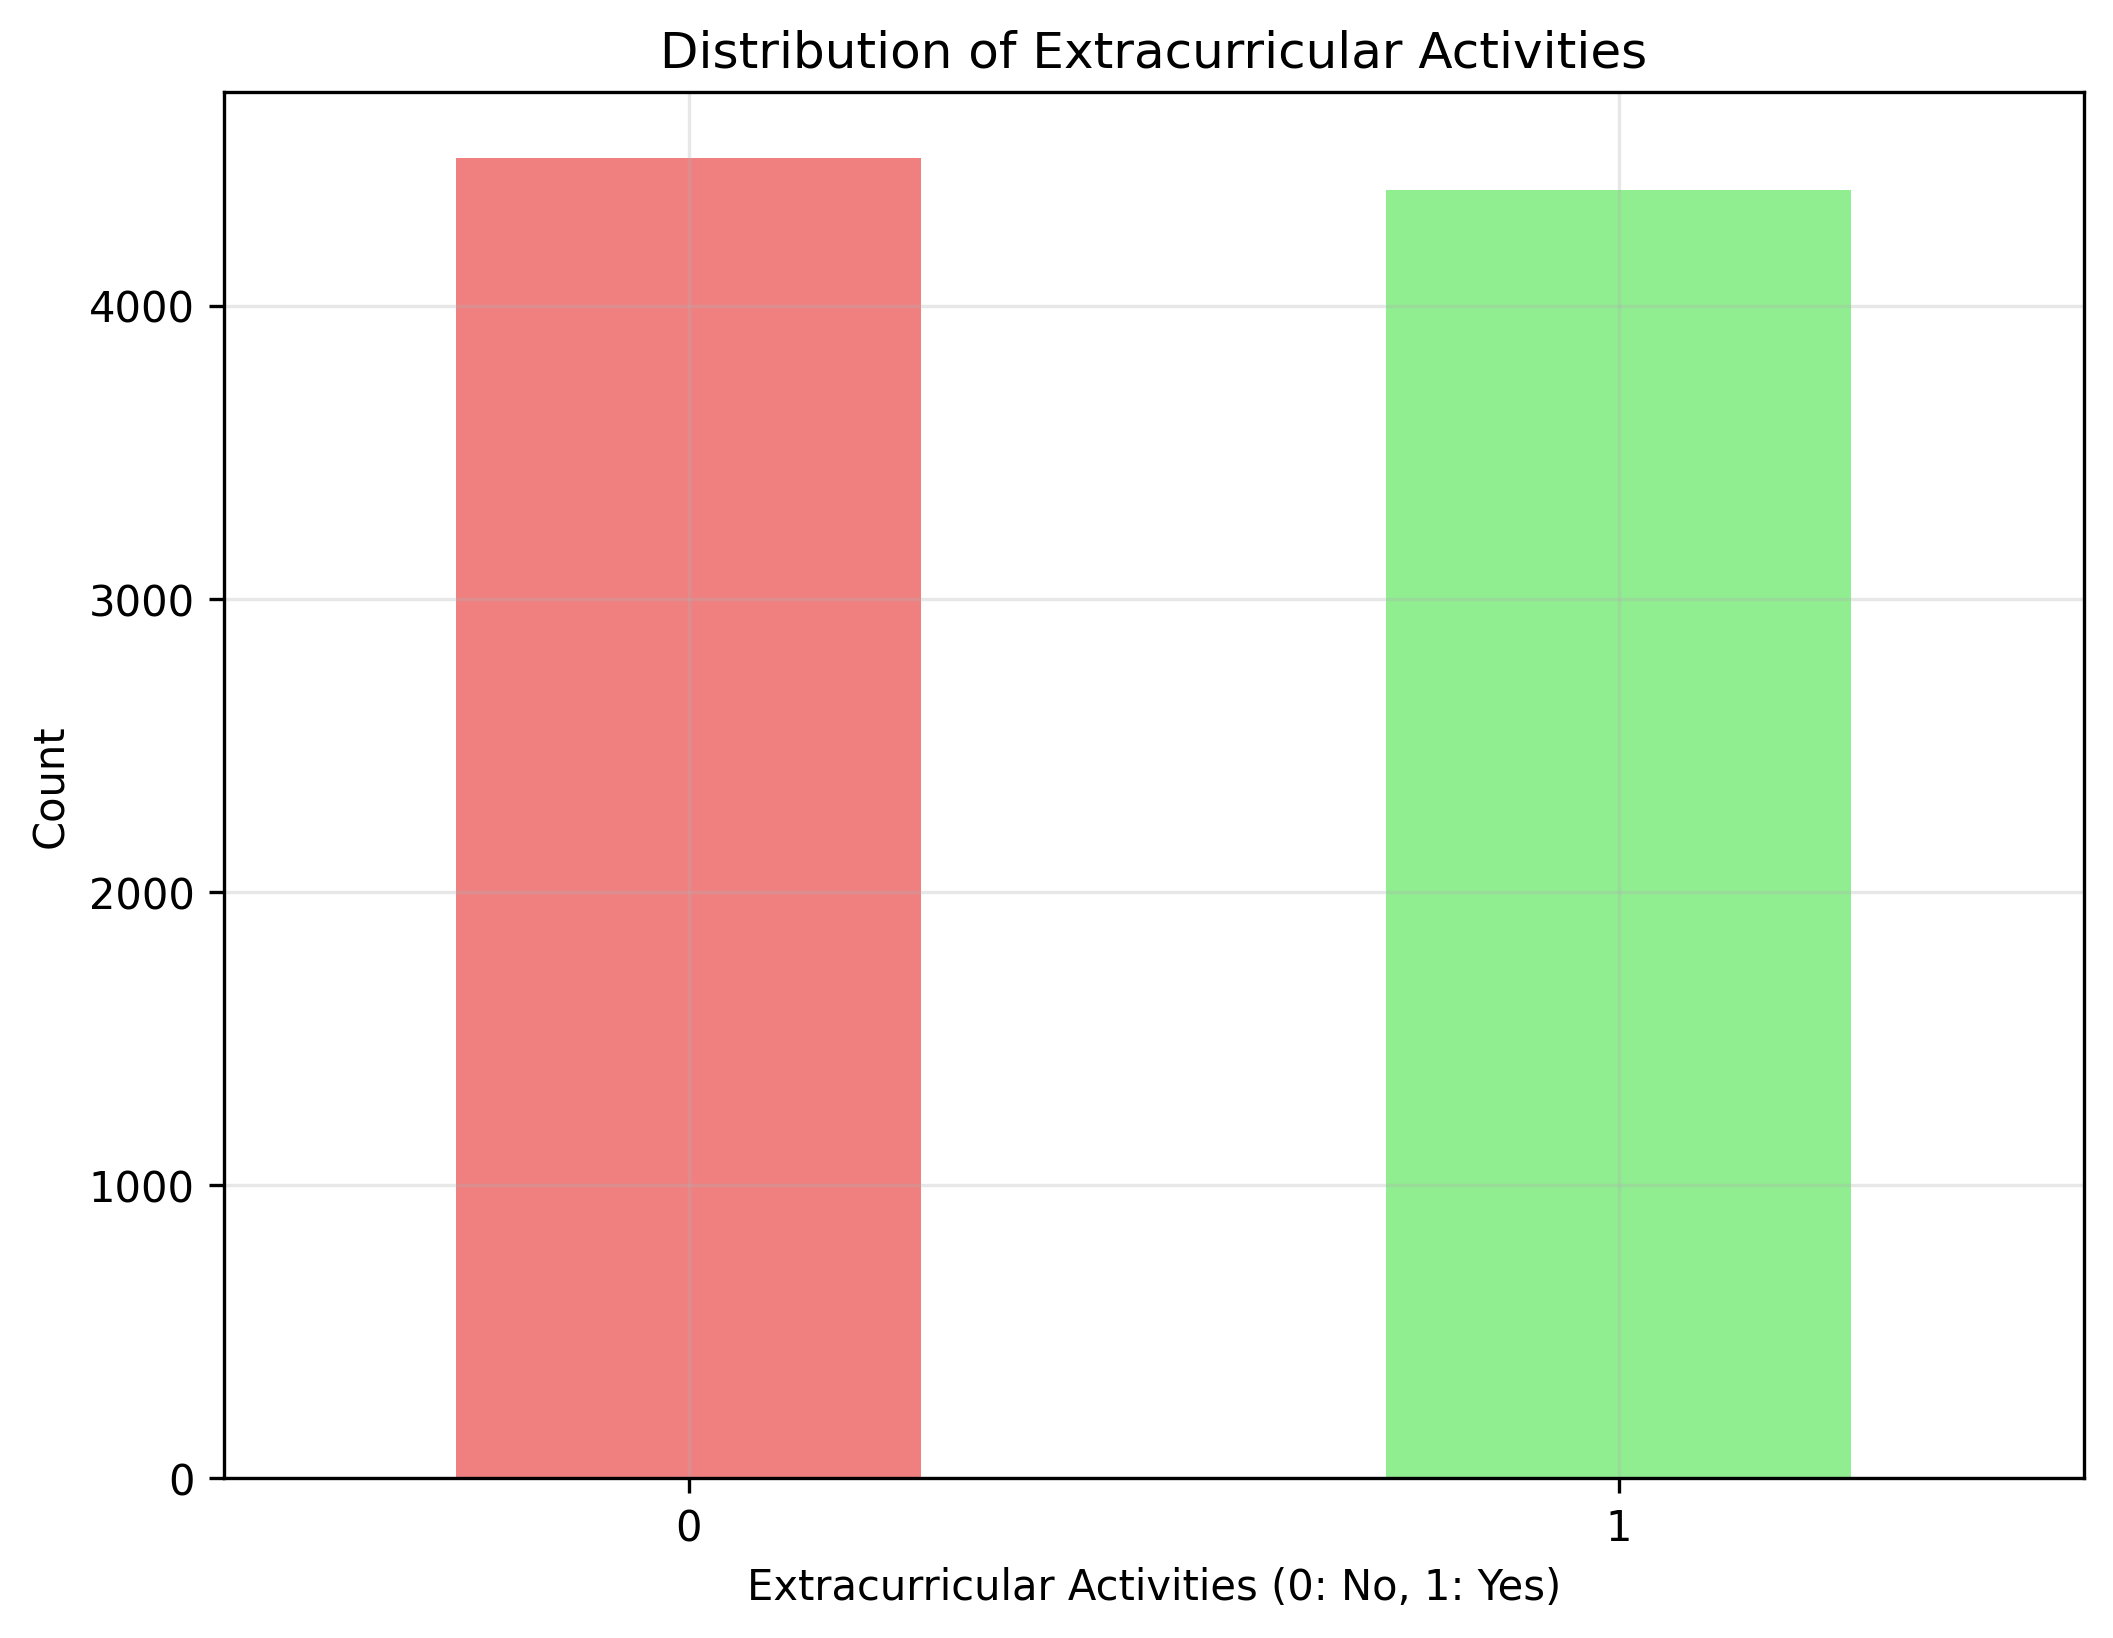
\includegraphics[width=0.7\textwidth]{imgs/figures/figure3_extracurricular_activities_distribution.png}
	\caption{Phân phối Hoạt động Ngoại khóa}
	\label{fig:extracurricular}
\end{figure}

\begin{itemize}
	\item \textbf{Nhận xét:}
	      \begin{itemize}
		      \item \textbf{Phân bố cân bằng}: Số lượng sinh viên tham gia và không tham gia hoạt động ngoại khóa gần như bằng nhau.
		      \item \textbf{Tính đại diện}: Sự cân bằng này đảm bảo dữ liệu có tính đại diện tốt, tránh thiên lệch trong phân tích.
	      \end{itemize}
\end{itemize}

\begin{figure}[H]
	\centering
	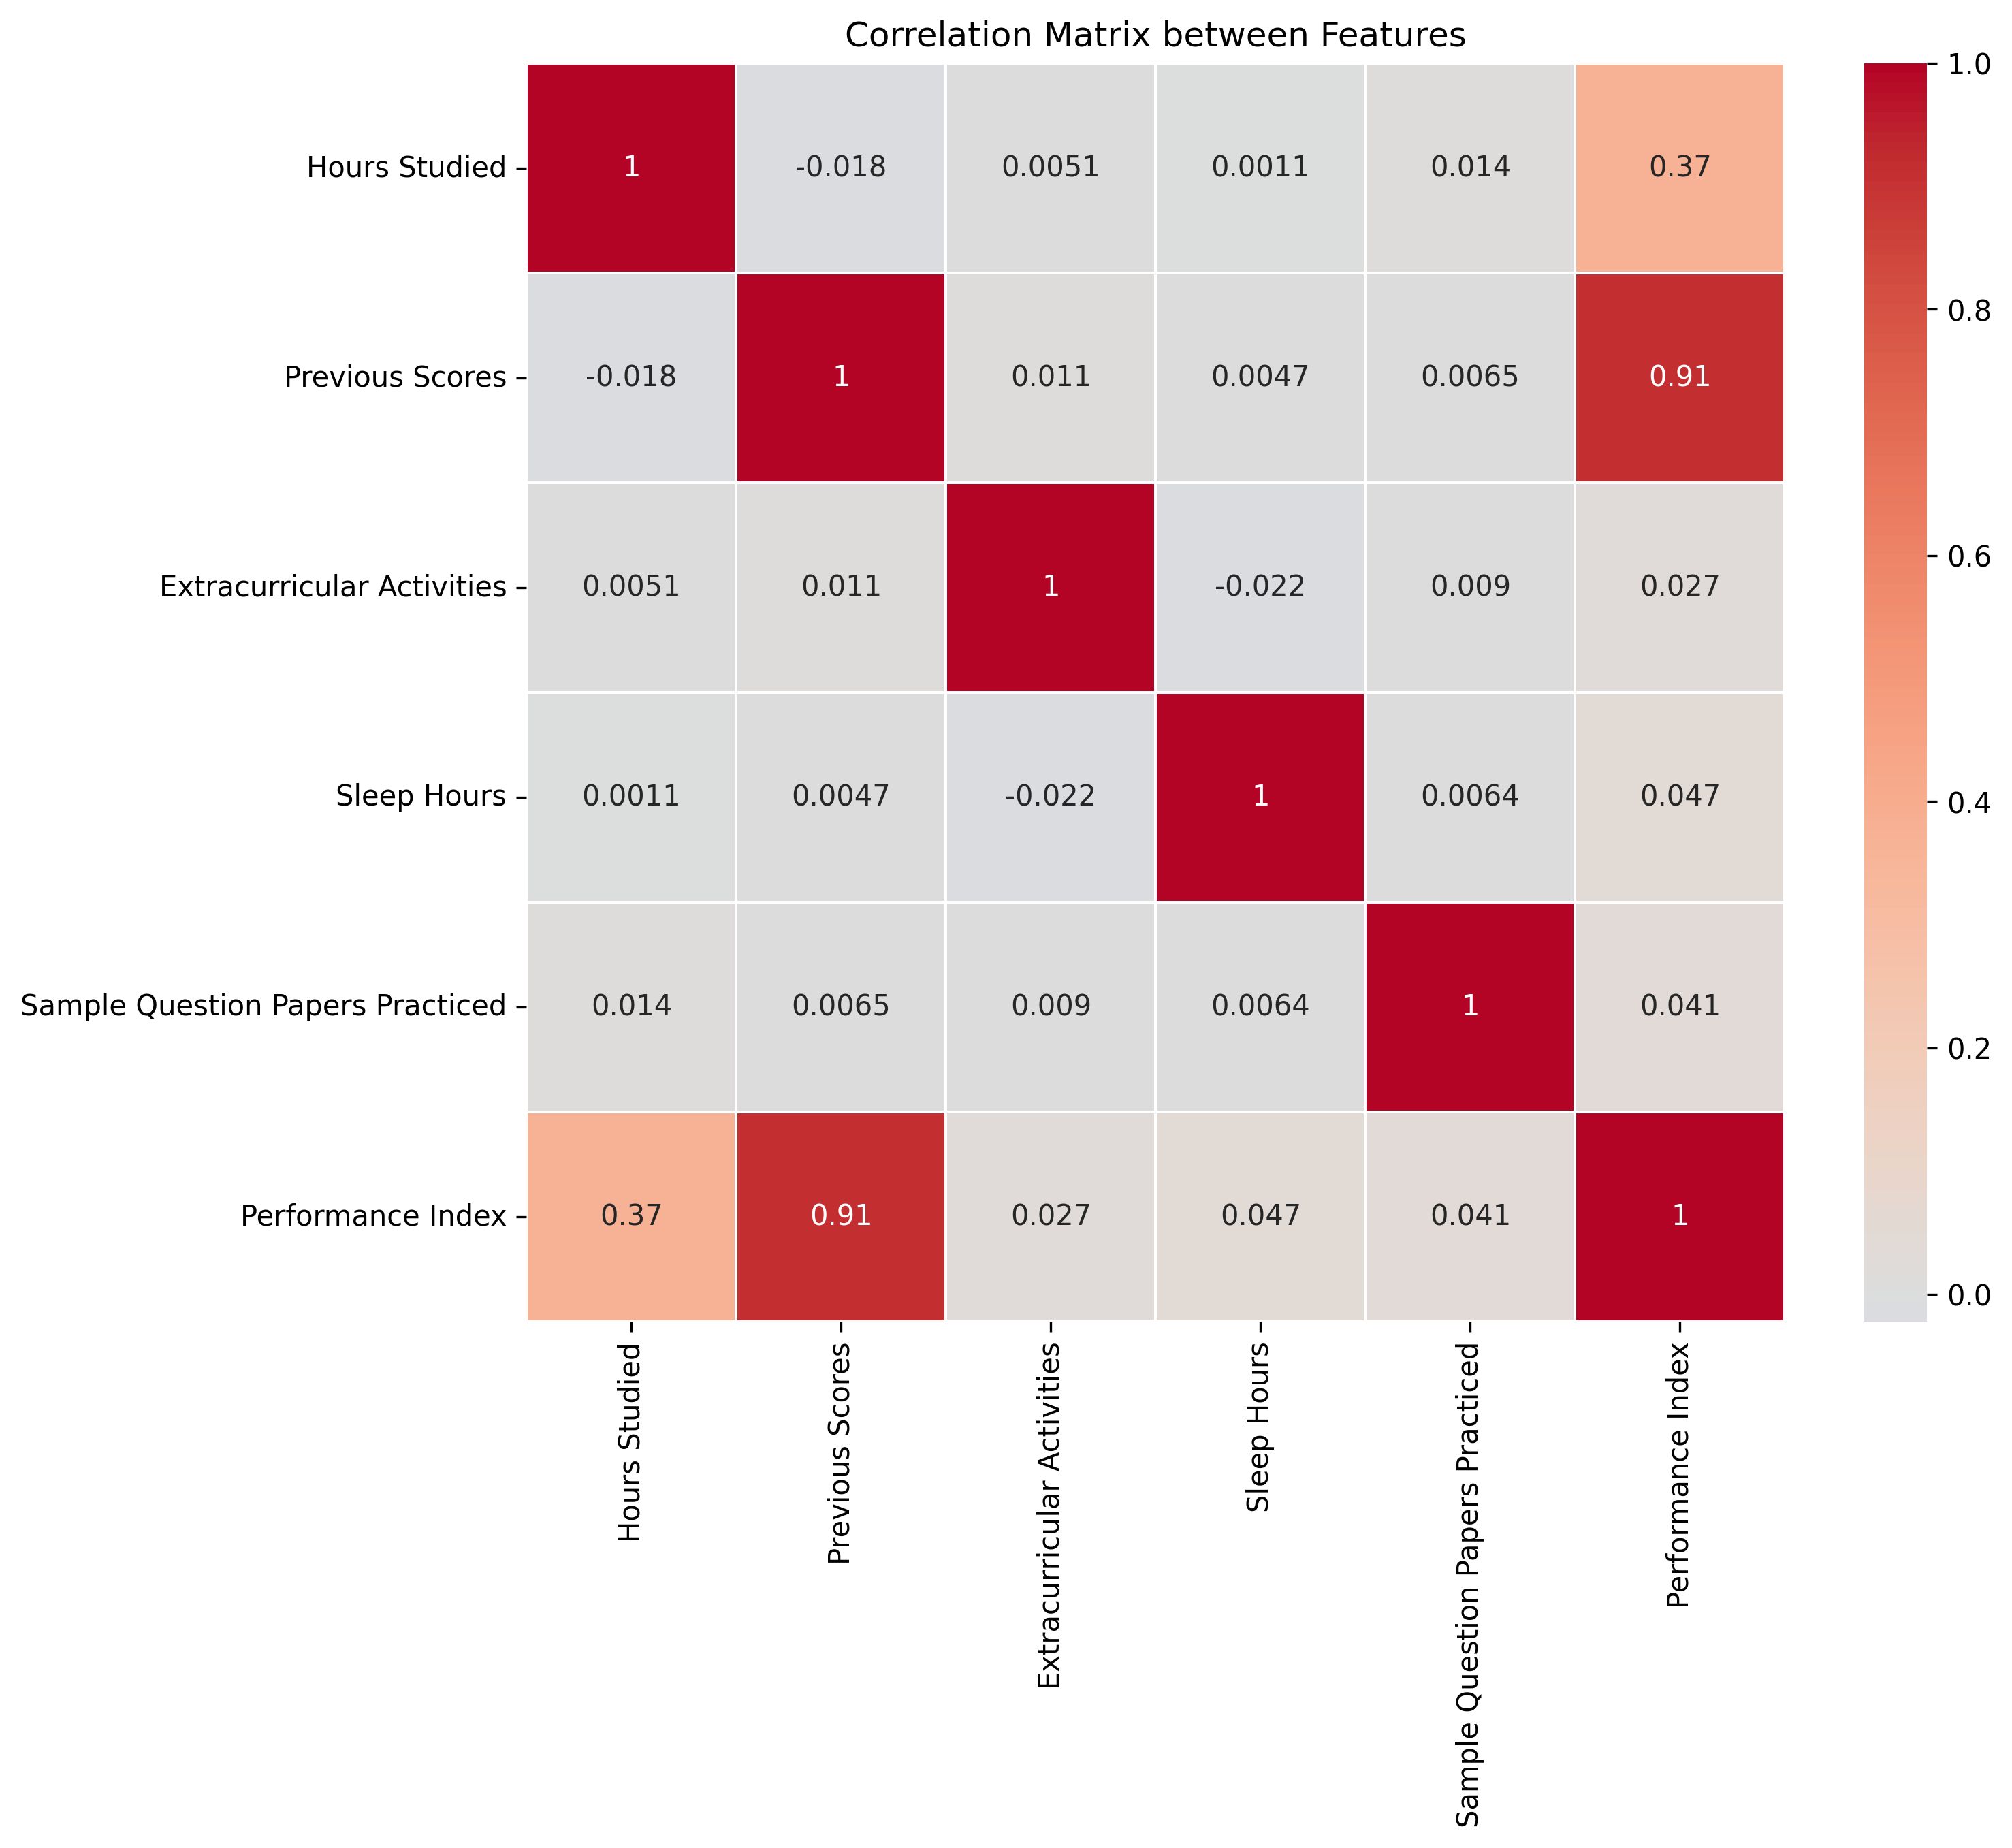
\includegraphics[width=0.9\textwidth]{imgs/figures/figure4_correlation_matrix.png}
	\caption{Ma trận tương quan giữa các đặc trưng}
	\label{fig:correlation}
\end{figure}

\begin{itemize}
	\item \textbf{Nhận xét:}
	      \begin{itemize}
		      \item Previous Scores có tương quan rất mạnh với Performance Index (0.91) → Điểm số trước đây dự đoán tốt hiệu suất.
		      \item Hours Studied có tương quan dương vừa phải với Performance Index (0.37) → Học nhiều giờ giúp cải thiện hiệu suất, nhưng không mạnh bằng điểm số trước.
		      \item Các biến khác (Extracurricular Activities, Sleep Hours, Sample Question Papers Practiced) hầu như không có tương quan đáng kể với Performance Index (< 0.05).
	      \end{itemize}
\end{itemize}

\begin{figure}[H]
	\centering
	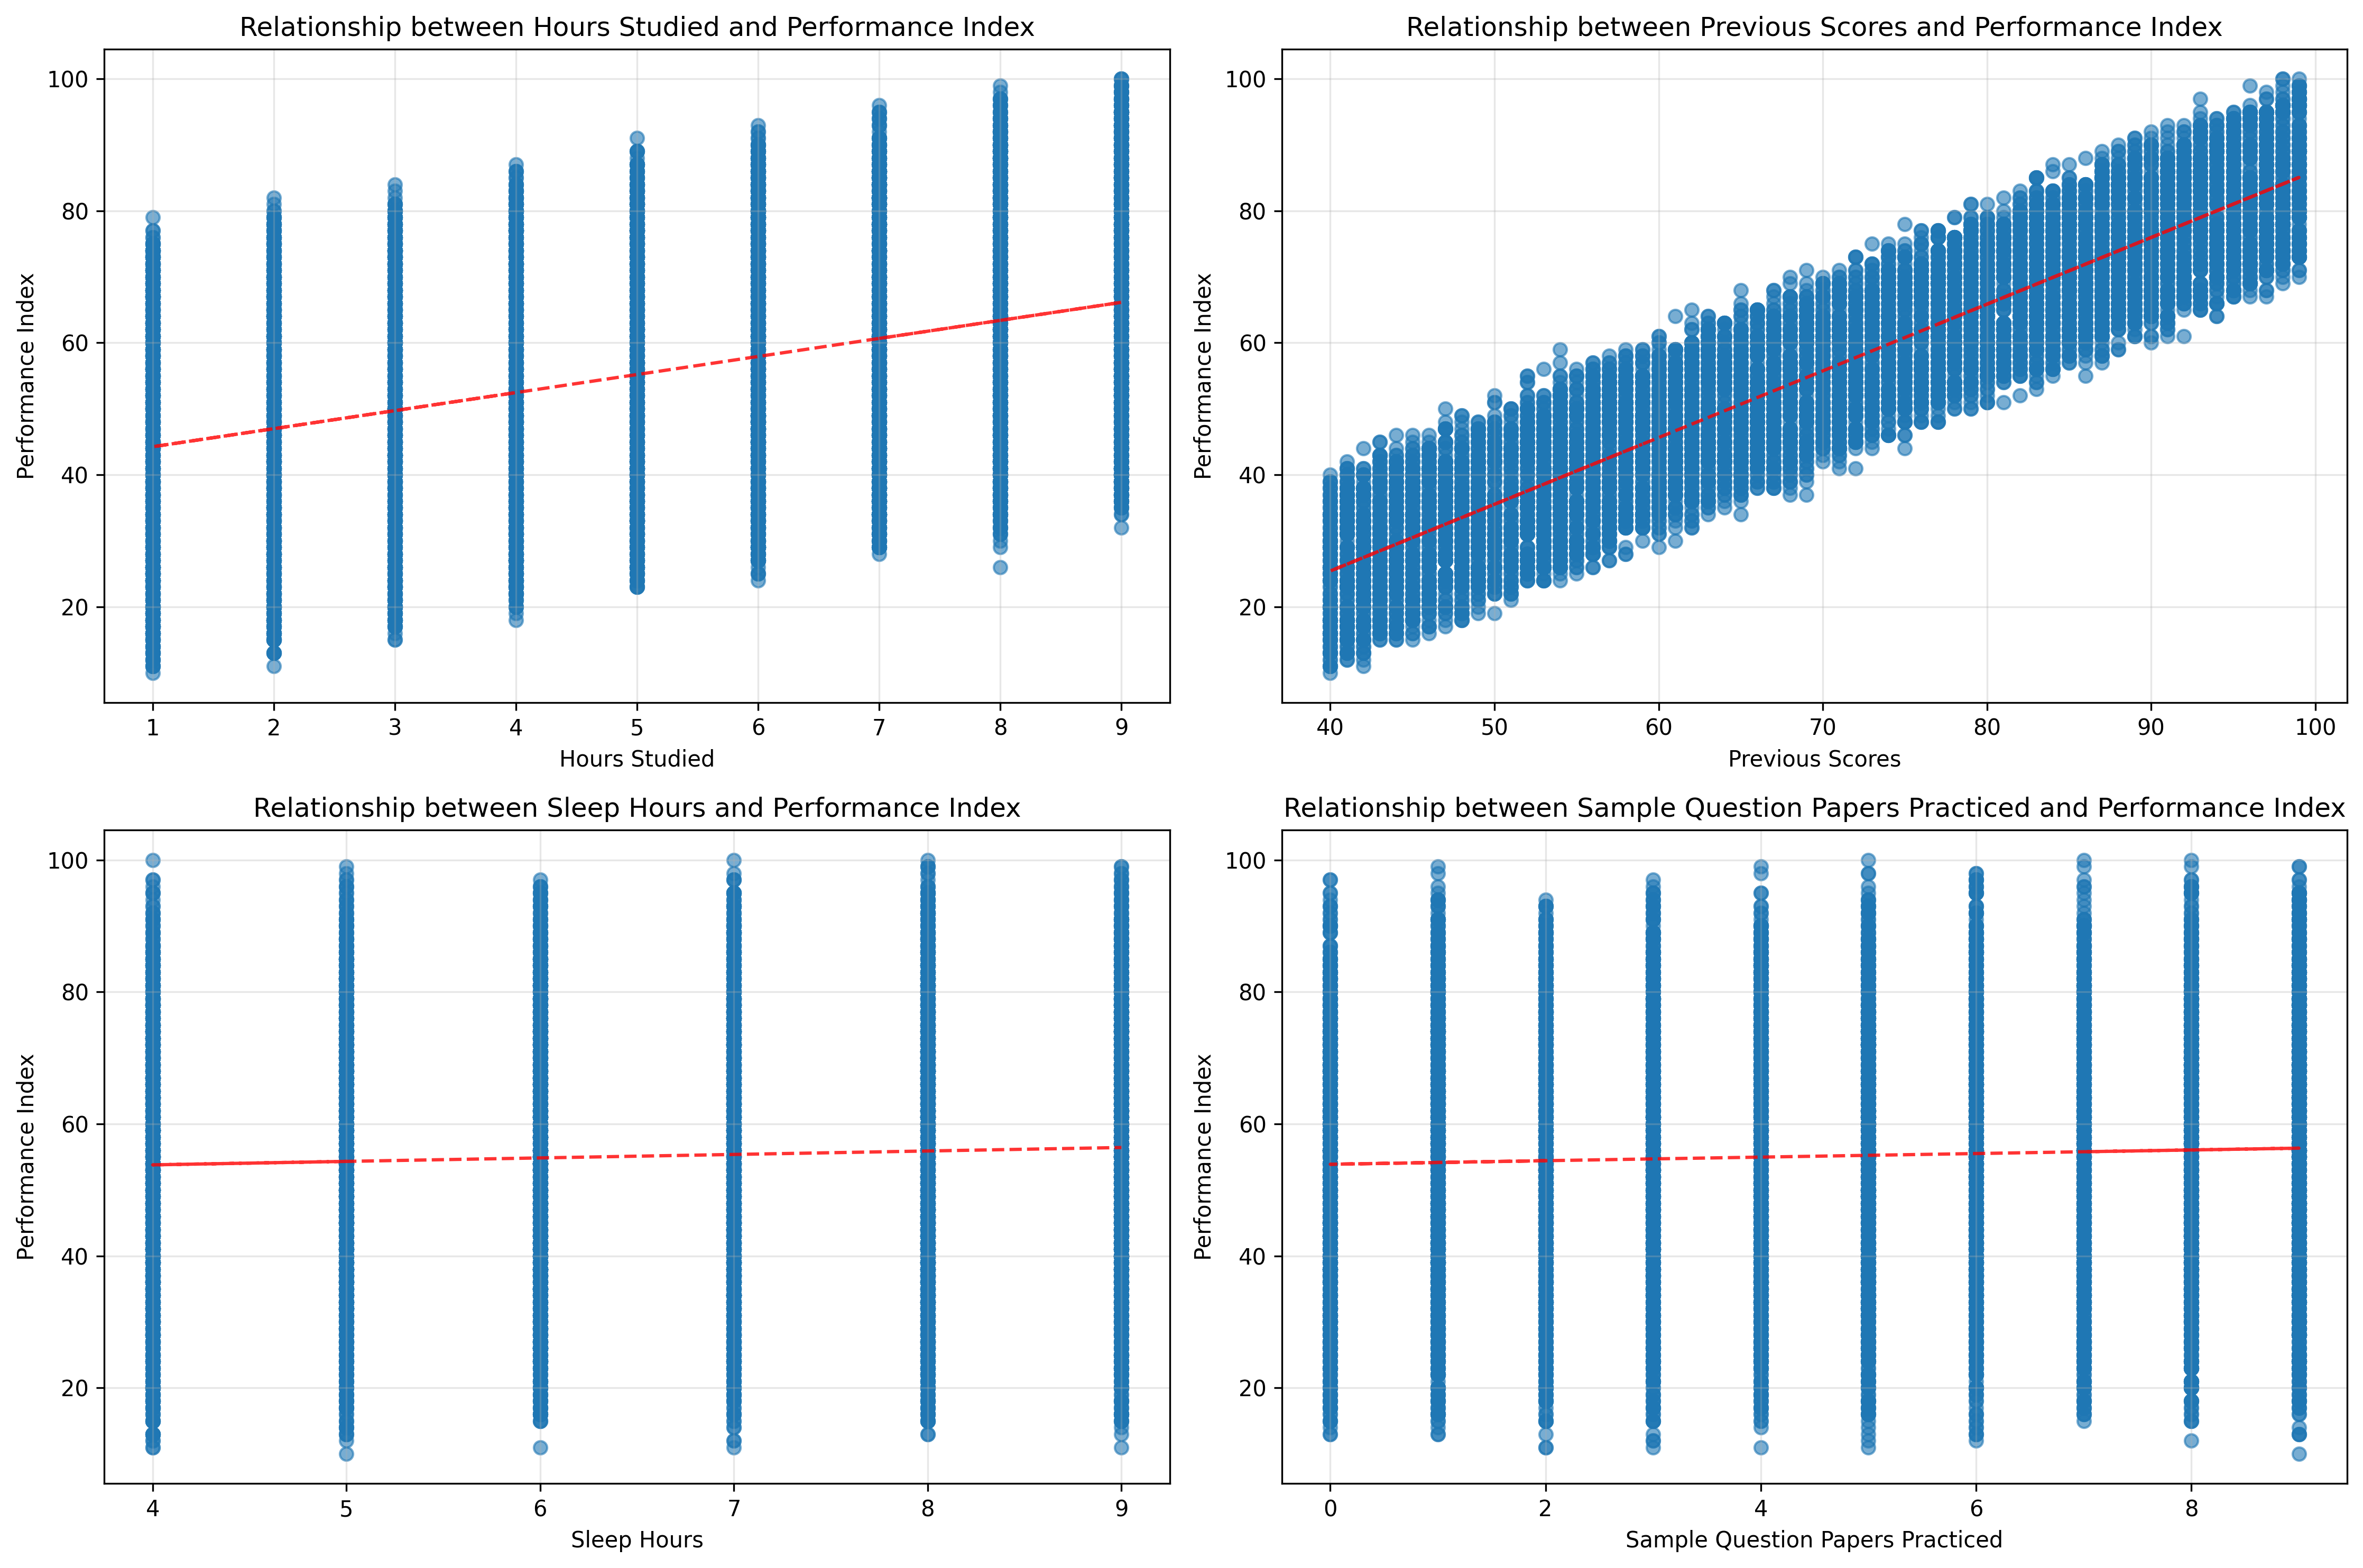
\includegraphics[width=0.9\textwidth]{imgs/figures/figure5_scatter_plots_relationships.png}
	\caption{Biểu đồ phân tán mối quan hệ với Performance Index}
	\label{fig:scatter}
\end{figure}

\begin{itemize}
	\item \textbf{Nhận xét:}
	      \begin{itemize}
		      \item \textbf{Previous Scores}: Có mối quan hệ tuyến tính mạnh và rõ ràng với Performance Index. Đường hồi quy cho thấy correlation coefficient cao, với sự phân bố dữ liệu khá sát đường thẳng.
		      \item \textbf{Hours Studied}: Mối quan hệ tuyến tính yếu hơn nhưng vẫn rõ ràng. Có xu hướng tăng nhẹ theo thời gian học, nhưng độ phân tán lớn hơn Previous Scores.
		      \item \textbf{Sleep Hours}: Mối quan hệ rất yếu hoặc không có correlation rõ ràng. Đường hồi quy gần như nằm ngang, cho thấy Sleep Hours ít ảnh hưởng đến Performance Index.
		      \item \textbf{Sample Question Papers Practiced}: Tương tự Sleep Hours, mối quan hệ rất yếu với đường hồi quy gần như nằm ngang, cho thấy việc luyện tập đề mẫu không có tác động mạnh đến hiệu suất tổng thể.
	      \end{itemize}
\end{itemize}

\begin{figure}[H]
	\centering
	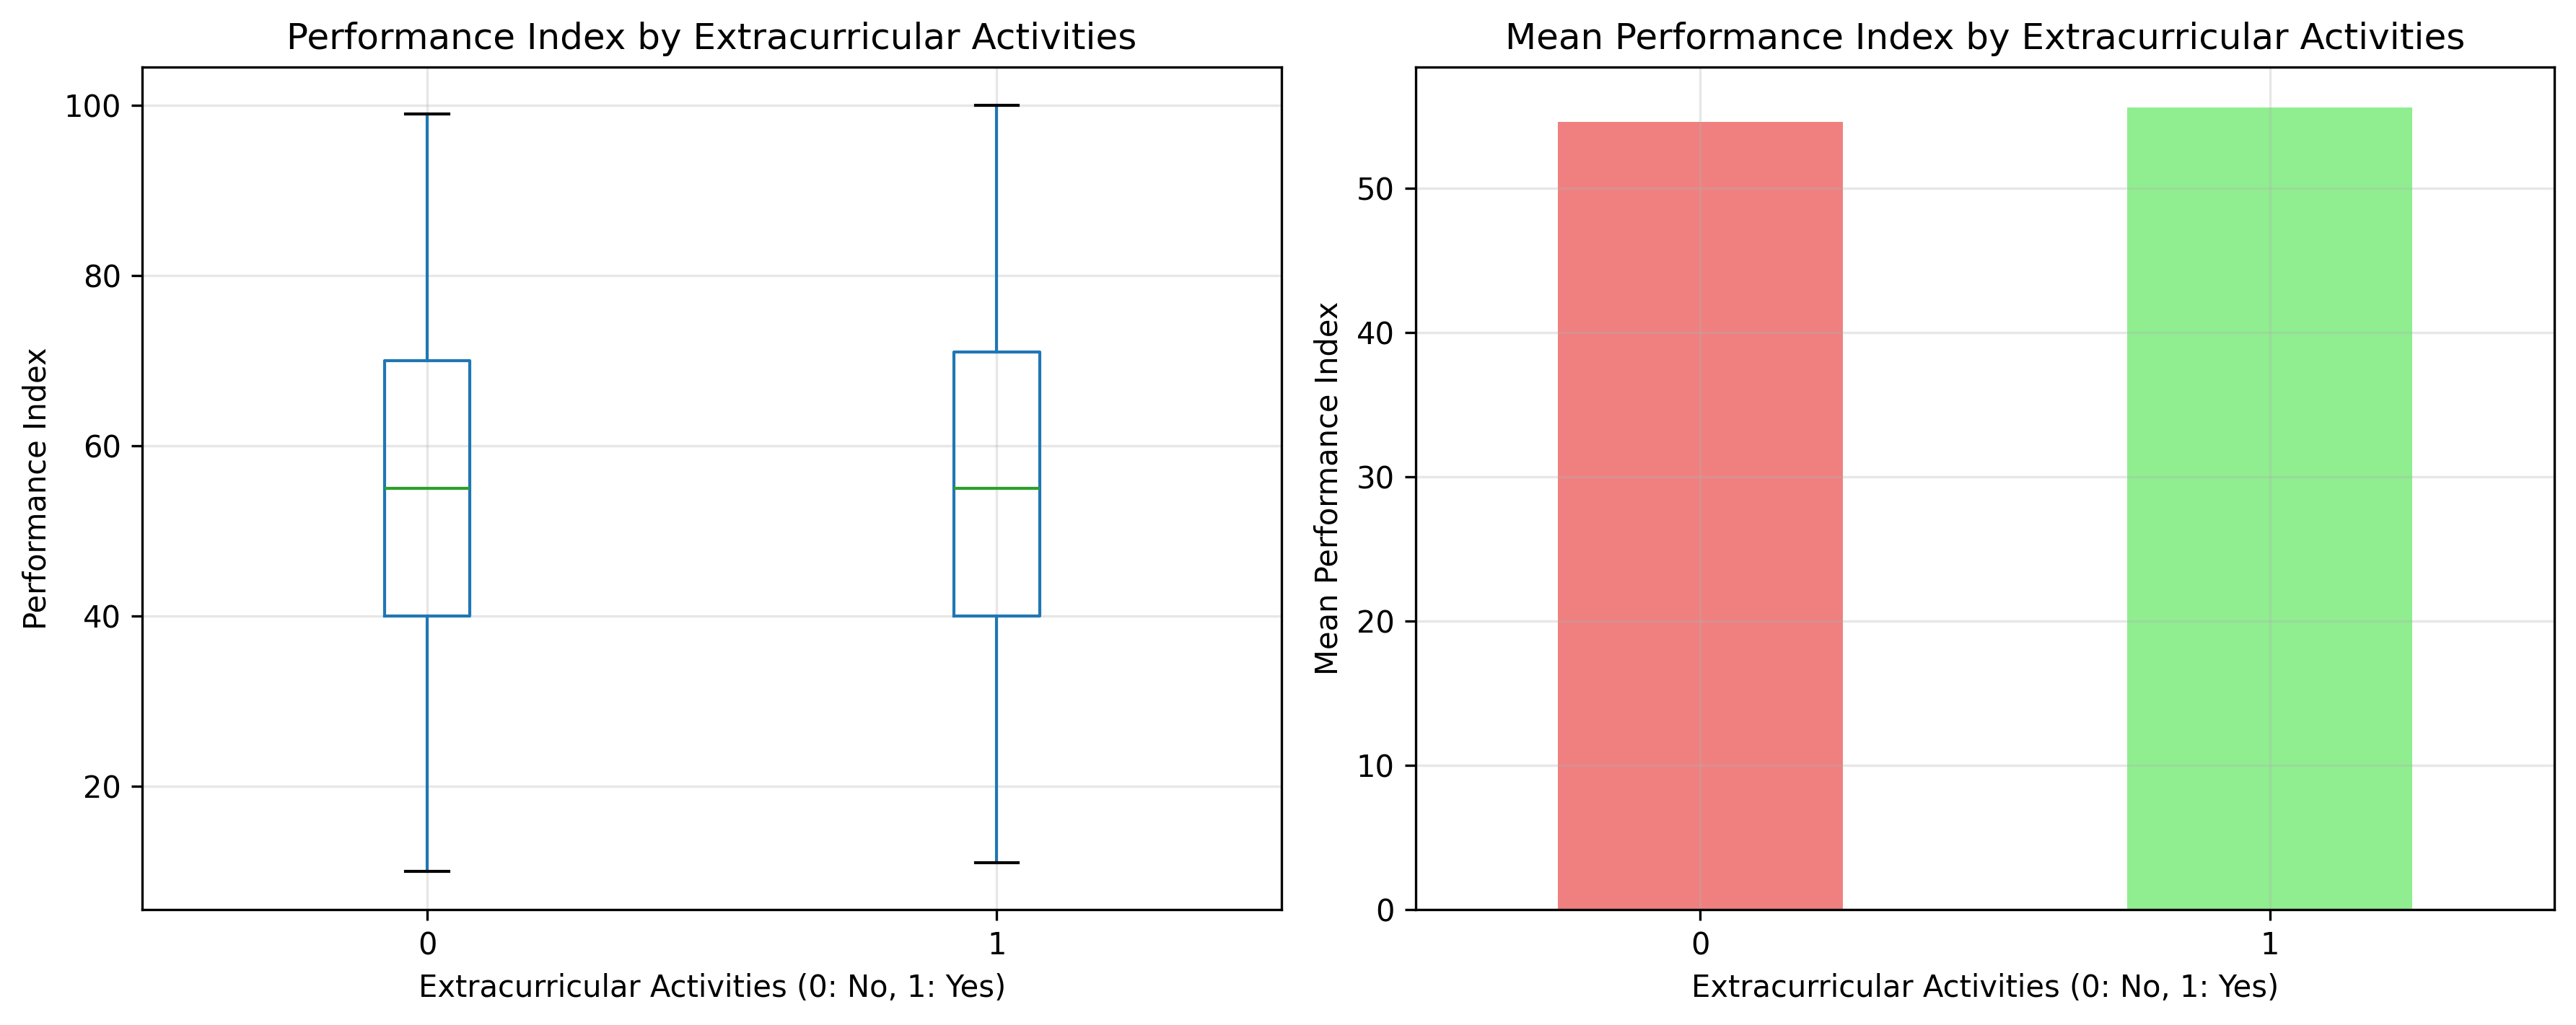
\includegraphics[width=0.9\textwidth]{imgs/figures/figure6_performance_by_extracurricular.png}
	\caption{So sánh hiệu suất theo hoạt động ngoại khóa}
	\label{fig:performance_comparison}
\end{figure}

\begin{itemize}
	\item \textbf{Nhận xét:}
	      \begin{itemize}
		      \item \textbf{Phân phối tương tự nhau}: Từ biểu đồ boxplot, cả hai nhóm (có và không có hoạt động ngoại khóa) đều có phân phối Performance Index khá tương đồng với median gần như bằng nhau (khoảng 55 điểm).
		      \item \textbf{Độ biến thiên tương đương}: Khoảng tứ phân vị (IQR) của cả hai nhóm gần như bằng nhau, cho thấy độ phân tán dữ liệu tương tự.
		      \item \textbf{Chênh lệch mean nhẹ}: Biểu đồ cột cho thấy sinh viên tham gia hoạt động ngoại khóa (nhóm 1) có điểm trung bình cao hơn một chút so với nhóm không tham gia (nhóm 0), nhưng sự khác biệt không lớn (khoảng 1-2 điểm).
		      \item \textbf{Tác động hạn chế}: Mặc dù có sự khác biệt về mean, nhưng sự chồng lấn lớn giữa hai phân phối cho thấy hoạt động ngoại khóa có tác động tích cực nhưng không quá mạnh đến hiệu suất học tập.
	      \end{itemize}
\end{itemize}

\subsection{Kết quả các Mô hình Hồi quy Tuyến tính}

\subsubsection{Yêu cầu 2a: Mô hình 5 đặc trưng}

\textbf{Công thức mô hình}:
\begin{align}
	\text{Performance} & = -33.961 + 2.852 \times \text{Hours Studied} \nonumber          \\
	                   & \quad + 1.018 \times \text{Previous Scores} \nonumber            \\
	                   & \quad + 0.606 \times \text{Extracurricular Activities} \nonumber \\
	                   & \quad + 0.473 \times \text{Sleep Hours} \nonumber                \\
	                   & \quad + 0.192 \times \text{Sample Question Papers}
\end{align}

\textbf{Kết quả đánh giá}:
\begin{itemize}
	\item \textbf{MSE trên tập kiểm tra}: 4.092356
	\item \textbf{Nhận xét}: Mô hình sử dụng toàn bộ 5 đặc trưng cho kết quả khá tốt, với Previous Scores và Hours Studied có trọng số cao nhất.
\end{itemize}

\subsubsection{Yêu cầu 2b: Mô hình đặc trưng tốt nhất}

\textbf{Kết quả k-fold Cross Validation}:

\begin{table}[H]
	\centering
	\begin{tabular}{|c|l|c|}
		\hline
		\textbf{STT} & \textbf{Mô hình với 1 đặc trưng} & \textbf{MSE} \\
		\hline
		1            & Hours Studied                    & 317.510929   \\
		\hline
		2            & Previous Scores                  & 60.141086    \\
		\hline
		3            & Extracurricular Activities       & 367.670027   \\
		\hline
		4            & Sleep Hours                      & 367.287602   \\
		\hline
		5            & Sample Question Papers Practiced & 367.485440   \\
		\hline
	\end{tabular}
	\caption{Kết quả Cross Validation cho mô hình 1 đặc trưng}
	\label{tab:single_feature}
\end{table}

\textbf{Đặc trưng tốt nhất}: Previous Scores với MSE = 60.141086

\textbf{Công thức mô hình}:
\begin{equation}
	\text{Performance} = -15.015 + 1.011 \times \text{Previous Scores}
\end{equation}

\textbf{Kết quả đánh giá}:
\begin{itemize}
	\item \textbf{MSE trên tập kiểm tra}: 58.906757
	\item \textbf{Giải thích}: Previous Scores là đặc trưng quan trọng nhất vì nó phản ánh trực tiếp năng lực học tập trước đó của sinh viên, có tương quan mạnh với kết quả hiện tại.
\end{itemize}

\subsubsection{Yêu cầu 2c: Mô hình tùy chỉnh}

\textbf{Các mô hình được thiết kế}:

\begin{table}[H]
	\centering
	\begin{tabular}{|c|l|c|}
		\hline
		\textbf{STT} & \textbf{Mô hình}                & \textbf{MSE} \\
		\hline
		1            & 2 đặc trưng tốt nhất            & 5.220514     \\
		\hline
		2            & 3 đặc trưng tốt nhất            & 5.136711     \\
		\hline
		3            & Đặc trưng đa thức               & 60.180196    \\
		\hline
		4            & Đặc trưng chuẩn hóa z-score     & 5.220514     \\
		\hline
		5            & Đặc trưng tương tác và kỹ thuật & 18.505961    \\
		\hline
	\end{tabular}
	\caption{Kết quả Cross Validation cho các mô hình tùy chỉnh}
	\label{tab:custom_models}
\end{table}

\textbf{Mô hình tốt nhất}: Model 2 (Top 3 features) với MSE = 5.136711

\textbf{Công thức mô hình}:
\begin{align}
	\text{Performance} & = -30.019 + 2.855 \times \text{Hours Studied} \nonumber \\
	                   & \quad + 1.018 \times \text{Previous Scores} \nonumber   \\
	                   & \quad + 0.580 \times \text{Extracurricular Activities}
\end{align}

\textbf{Kết quả đánh giá}:
\begin{itemize}
	\item \textbf{MSE trên tập kiểm tra}: 5.273269
	\item \textbf{Giải thích}: Mô hình kết hợp 3 đặc trưng quan trọng nhất cho kết quả tốt nhất, loại bỏ được nhiễu từ các đặc trưng ít quan trọng.
\end{itemize}

\subsection{Phân tích và So sánh các Mô hình}

\subsubsection{Bảng tổng hợp kết quả}

\begin{table}[H]
	\centering
	\begin{tabular}{|l|c|c|}
		\hline
		\textbf{Mô hình}                & \textbf{MSE Cross Validation} & \textbf{MSE Test} \\
		\hline
		Mô hình 5 đặc trưng (2a)        & -                             & 4.092356          \\
		\hline
		Đặc trưng tốt nhất (2b)         & 60.141086                     & 58.906757         \\
		\hline
		Mô hình tùy chỉnh tốt nhất (2c) & 5.136711                      & 5.273269          \\
		\hline
	\end{tabular}
	\caption{So sánh kết quả các mô hình}
	\label{tab:model_comparison}
\end{table}

\subsubsection{Nhận xét về hiệu suất}

\textbf{Thứ tự hiệu suất (từ tốt đến kém)}:
\begin{enumerate}
	\item \textbf{Mô hình 5 đặc trưng (2a)}: MSE = 4.092356
	\item \textbf{Mô hình tùy chỉnh tốt nhất (2c)}: MSE = 5.273269
	\item \textbf{Đặc trưng tốt nhất (2b)}: MSE = 58.906757
\end{enumerate}

\textbf{Phân tích hiệu suất}:
\begin{itemize}
	\item Mô hình 5 đặc trưng (2a) đạt hiệu suất tốt nhất với MSE thấp nhất, cho thấy sự đóng góp tích cực của tất cả các đặc trưng
	\item Mô hình tùy chỉnh (2c) có hiệu suất tốt thứ hai, chứng tỏ việc lựa chọn đặc trưng thông minh có thể cạnh tranh với mô hình đầy đủ
	\item Mô hình 1 đặc trưng (2b) có hiệu suất thấp nhất do hạn chế thông tin đầu vào
\end{itemize}

\subsection{Kết luận cuối cùng}
Những yếu tố quan trọng ảnh hưởng đến thành tích học tập theo thứ tự ưu tiên:
\begin{enumerate}
	\item \textbf{Previous Scores}: Yếu tố quan trọng nhất, phản ánh nền tảng kiến thức
	\item \textbf{Hours Studied}: Thời gian học tập có tác động mạnh đến kết quả
	\item \textbf{Extracurricular Activities}: Hoạt động ngoại khóa góp phần nâng cao hiệu suất học tập
	\item \textbf{Sleep Hours}: Có tác động nhưng không mạnh bằng các yếu tố trên
	\item \textbf{Sample Question Papers Practiced}: Tác động thấp nhất trong các yếu tố được khảo sát
\end{enumerate}



